\documentclass{beamer}

\mode<presentation> {
	\usetheme{Madrid}
}

\usepackage{graphicx}
\usepackage{booktabs}
\usepackage[T2A]{fontenc}
\usepackage[utf8]{inputenc}
\usepackage[russian, english]{babel}
\usepackage{enumerate}
\usepackage{setspace}
\usepackage{listing}
\usepackage{appendixnumberbeamer}

\newenvironment{MyList}[1][4pt]{
	\begin{enumerate}[1.]
		\setlength{\parskip}{0pt}
		\setlength{\itemsep}{#1}
	}{       
	\end{enumerate}
}
\newenvironment{InnerMyList}[1][0pt]{
	\vspace*{-0.5em}
	\begin{enumerate}[a)]
		\setlength{\parskip}{#1}
		\setlength{\itemsep}{0pt}
	}{
	\end{enumerate}
}

%----------------------------------------------------------------------------------------
%	TITLE PAGE
%----------------------------------------------------------------------------------------

\title[Cross-Modal Retrieval]{Improving Textual-Visual Cross-Modal Retrieval with Visual Attention to Text}

\author[Григорий Бартош]{
	\textbf{Григорий Бартош}\\
	Руководитель: Шпильман Алексей Александрович
}
\institute[ВШЭ СПб]{НИУ ВШЭ СПб}
\date[28.05.2019]{Вторник, 28 мая 2019 года}

\begin{document}
	
\begin{frame}
	\titlepage
\end{frame}

\begin{frame}
	\frametitle{Overview}
	\tableofcontents
\end{frame}

%----------------------------------------------------------------------------------------
%	PRESENTATION SLIDES
%----------------------------------------------------------------------------------------

%------------------------------------------------
\section{Постановка задачи}
%------------------------------------------------

\begin{frame}
	\frametitle{Постановка задачи}
	\begin{columns}[c]
		\column{.5\textwidth}
		\textbf{Cross-Modal Retrieval:}
		\begin{itemize}
			\item Есть объекты типа \textbf{A}
			\item Дан запрос --- объект типа \textbf{B}
			\item Найти наиболее подходящие объекты типа \textbf{A}
		\end{itemize}
	
		\textbf{Желаемое:}
		\centerline{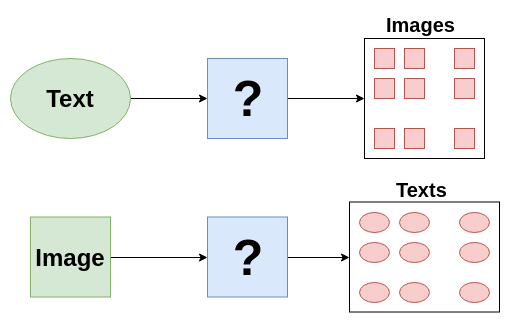
\includegraphics[scale=0.28]{images/desired.png}}
		
		\column{.5\textwidth}
		\centerline{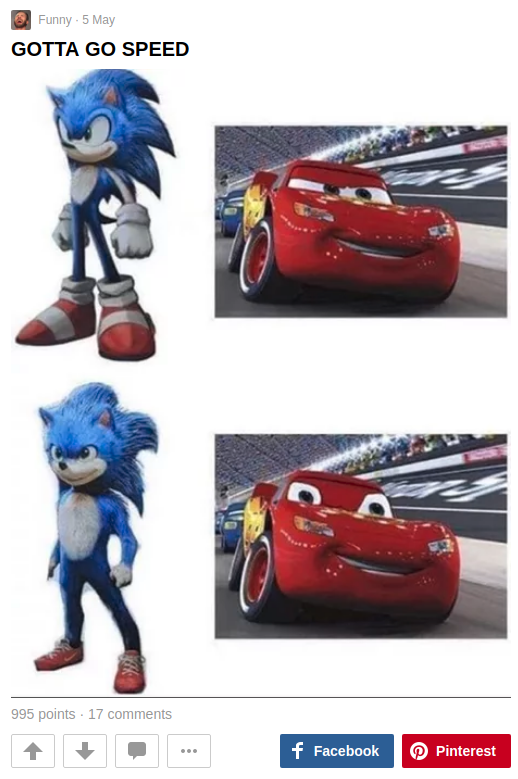
\includegraphics[scale=0.28]{images/meme.png}}
	\end{columns}
\end{frame}

%------------------------------------------------
\section{Обзор существующих решений}
%------------------------------------------------

\begin{frame}
	\frametitle{Обзор существующих решений}
	\textbf{Три типа решений:}
	\begin{itemize}
		\item
		Модели, возвращающие близость картинки и текста.
		
		\item
		Модели, строящие эмбеддинги в общем скрытом пространстве.
		
		\item
		Модели, хеширующие объекты.
	\end{itemize}
	
	\textbf{Проблемы:}
	\begin{itemize}
		\item
		Слабые текстовые модели.
		
		\item
		Равноправность текста и изображения.
		
		\item
		Ответ за линейное время или непроверенный ответ.
	\end{itemize}
	
	\centerline{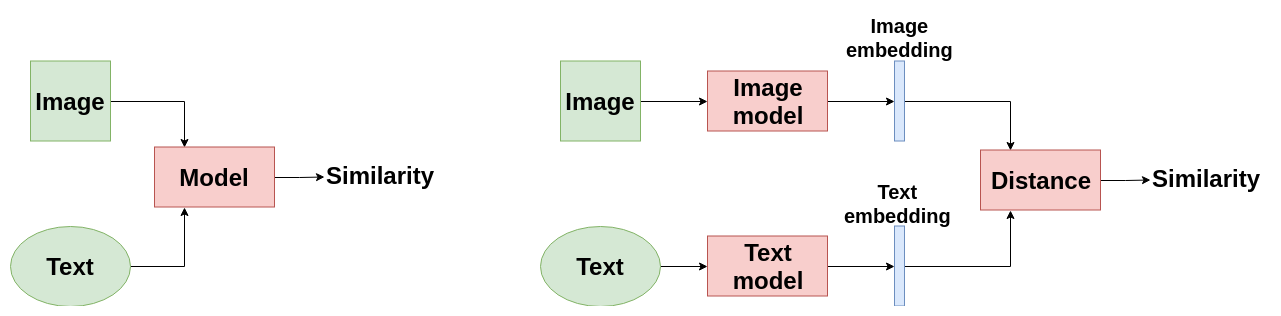
\includegraphics[scale=0.27]{images/solution_types.png}}
\end{frame}

%------------------------------------------------
\section{Решение}
\subsection{Данные и оценка модели}
%------------------------------------------------

\begin{frame}
	\frametitle{Решение: Данные и оценка модели}
	\begin{columns}[c]
		\column{.4\textwidth}
		\textbf{Датасет:}
		\begin{itemize}
			\item
			\textit{MS COCO 2014}
			
			\item
			train --- 82,783 изображения
			
			\item
			validation --- 40,504 изображения
			
			\item
			Каждая картинка имеет 5 текстовых описаний
		\end{itemize}
		
		\column{.6\textwidth}
		\centerline{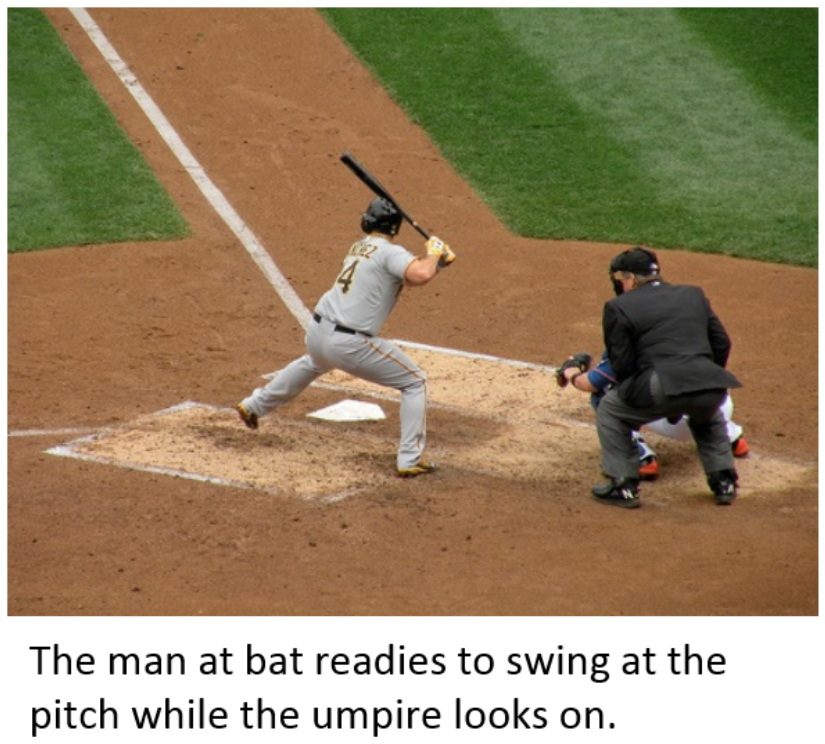
\includegraphics[scale=0.2]{images/mscoco_sample.png}}
	\end{columns}

	\textbf{Оценка модели:}
	\begin{itemize}
		\item
		Берем объект \textbf{a} типа \textbf{A} и \textbf{X} из $1000$ объектов типа \textbf{B}.
		
		\item
		Делаем $sort($ \textbf{X} $, x \rightarrow dist(x, $ \textbf{a} $))$.
		
		\item
		Смотрим на положение парного для \textbf{a} элемента в упорядоченном множестве.
	\end{itemize}
\end{frame}

%------------------------------------------------
\subsection{Архитектура}
%------------------------------------------------

\begin{frame}
	\frametitle{Решение: Архитектура}
	\centerline{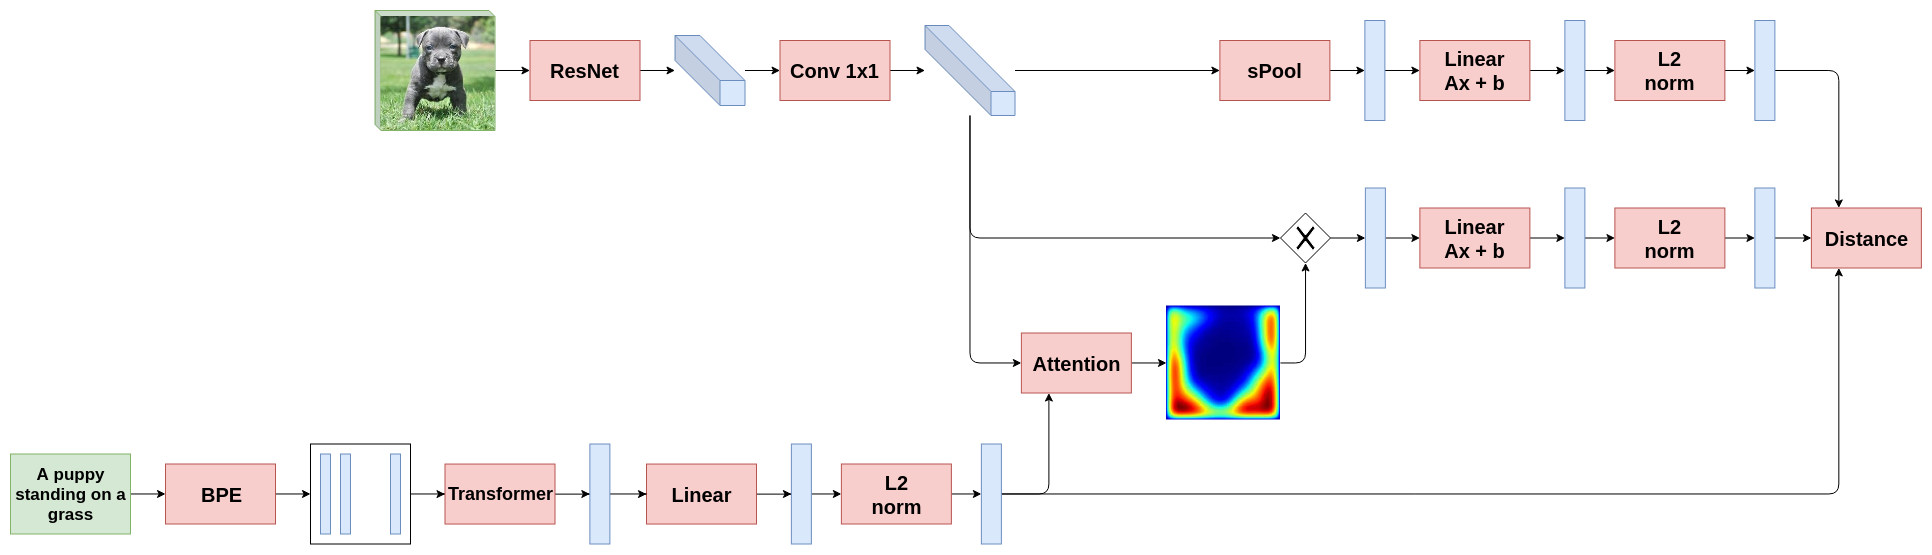
\includegraphics[scale=0.18]{images/architecture.png}}
\end{frame}

\begin{frame}
	\frametitle{Решение: Архитектура attention}
	\centerline{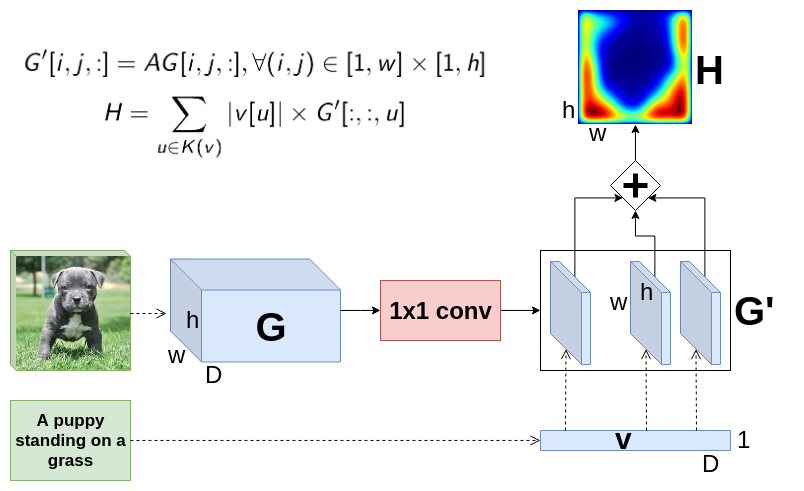
\includegraphics[scale=0.4]{images/architecture_attention.png}}
\end{frame}

%------------------------------------------------
\subsection{Обучение}
%------------------------------------------------

\begin{frame}
	\frametitle{Решение: Обучение}	
	\textbf{Triplet loss:}
	$$\mathcal{L}(\Theta, B) = \frac{1}{|B|} \sum_{n \in B} \left( \sum_{m \in B} loss(x_n, v_n, v_m) + \sum_{m \in B} loss(v_n, x_n, x_m) \right)$$
	$$loss(y, z, z') = \max(0, \alpha - \langle y, z \rangle + \langle y, z' \rangle)$$
	
	\textbf{Hard Negative Triplet loss:}
	$$\mathcal{L}(\Theta, B) = \frac{1}{|B|} \sum_{n \in B} \left( \max_{m \in B} loss(x_n, v_n, v_m) + \max_{m \in B} loss(v_n, x_n, x_m) \right)$$
	
	\begin{columns}[c]
		\column{.5\textwidth}
		$\Theta$ --- параметры модели\\
		$B$ --- батч\\
		
		\column{.5\textwidth}
		$x_i$ --- эмбеддинг изображения\\
		$v_i$ --- эмбеддинг текста\\
	\end{columns}
\end{frame}

%------------------------------------------------
\subsection{Результаты}
%------------------------------------------------

\begin{frame}
	\frametitle{Решение: Результаты}
	\begin{table}
		\begin{tabular}{l c c c c c c c c}
			\toprule
			\textbf{Text} & \textbf{train} & \textbf{image} & \multicolumn{3}{c}{caption retrieval} & \multicolumn{3}{c}{image retrieval} \\
			\textbf{model} & \textbf{middle} & \textbf{head} & \textbf{R@1} & \textbf{R@5} & \textbf{R@10} & \textbf{R@1} & \textbf{R@5} & \textbf{R@10}\\
			\midrule
			SRU     & - & base   & 12.2 & 37.2 & 50.6 &  7.6 & 18.2 & 22.6\\ 
			SRU     & - & middle & 11.6 & 35.7 & 49.6 &  7.6 & 18.0 & 22.4\\ 
			SRU     & + & base   & 22.9 & 48.8 & 63.5 & 15.2 & 30.0 & 41.6\\
			SRU     & + & middle & 22.0 & 47.9 & 62.8 & 16.7 & 31.4 & 43.1\\ 
			Transf. & - & base   & 38.6 & 68.1 & 79.7 & 31.6 & 63.1 & 76.1\\
			Transf. & - & middle & 34.0 & 64.0 & 76.5 & 30.5 & 62.0 & 75.4\\
			Transf. & + & base   & \textbf{40.8} & \textbf{70.3} & \textbf{81.5} & 32.4 & 63.9 & 77.1\\
			Transf. & + & middle & 39.4 & 68.9 & 80.6 & \textbf{33.5} & \textbf{64.6} & \textbf{77.5}\\
			\bottomrule
		\end{tabular}
	\end{table}
\end{frame}

%------------------------------------------------
\section{Итог}
%------------------------------------------------

\begin{frame}
	\frametitle{Итоги и выводы}
	\textbf{Итоги:}
	\begin{itemize}
		\item 
		Модель сильно выигрывает у state-of-the-art аналога на моих глобальных параметрах
		
		\item
		Можно на свое усмотрение склонять модель в сторону ускорения или увеличения точности для Image Retrieval
	\end{itemize}
	
	\textbf{Выводы:}
	\begin{itemize}
		\item
		Transformer сильнее SRU
		
		\item
		Усиление текстовой модели усиливает всю модель для Cross-Modal Retrieval
		
		\item
		Полезно обучать \textit{связь} объектов на более ранних этапах
	\end{itemize}
\end{frame}

%------------------------------------------------
\appendix

\begin{frame}
	\frametitle{Пример Heat Map}
	\centerline{
\includegraphics[scale=0.18]{images/example.jpg}}

	\begin{columns}[c]
		\column{.33333\textwidth}
		\centerline{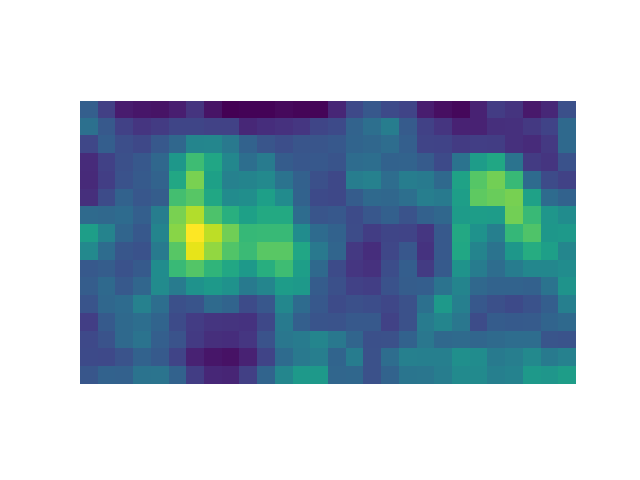
\includegraphics[scale=0.28]{images/example_1.png}}

		\column{.33333\textwidth}
		\centerline{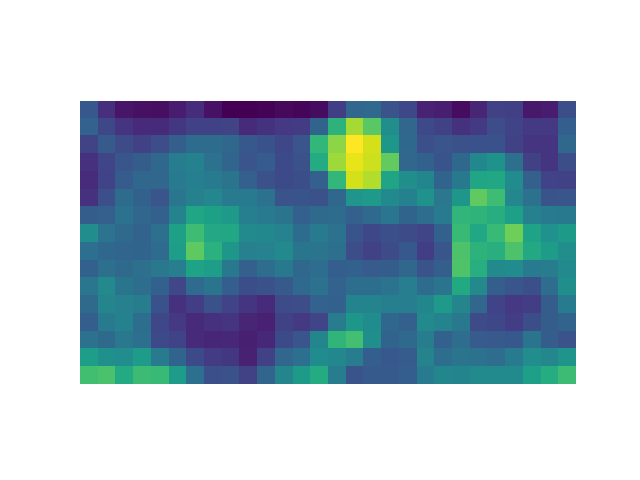
\includegraphics[scale=0.28]{images/example_2.png}}

		\column{.33333\textwidth}
		\centerline{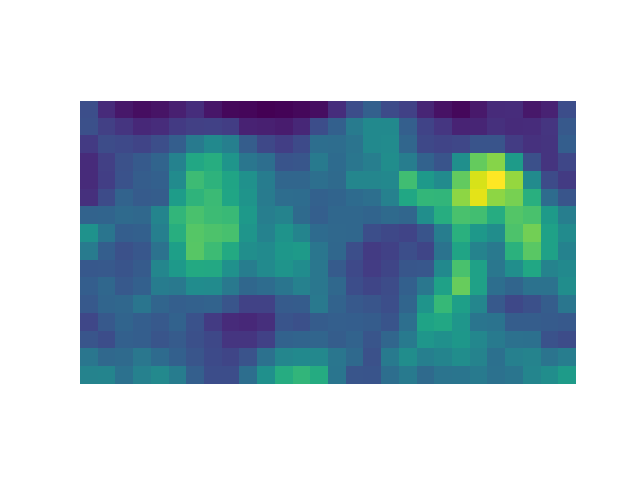
\includegraphics[scale=0.28]{images/example_3.png}}
	\end{columns}

	\begin{columns}[c]
		\column{.33333\textwidth}
		\centerline{\textit{a woman in red}}
		\centerline{\textit{dress}}

		\column{.33333\textwidth}
		\centerline{\textit{a man looking}}
		\centerline{\textit{left down}}

		\column{.33333\textwidth}
		\centerline{\textit{a woman standing}}
		\centerline{\textit{next to a man}}
	\end{columns}
\end{frame}

\begin{frame}
	\frametitle{Ссылки}
	\textbf{Модели первого типа:}
	\begin{itemize}
		\item
		\href{https://arxiv.org/abs/1611.05588}{\color{blue}{Instance-aware Image and Sentence Matching with Selective Multimodal LSTM}}
		
		\item
		\href{https://arxiv.org/abs/1708.04776}{\color{blue}{Modality-specific Cross-modal Similarity Measurement with Recurrent Attention Network}}
	\end{itemize}

	\textbf{Модели второго типа:}
	\begin{itemize}
		\item
		\href{https://arxiv.org/abs/1711.05535}{\color{blue}{Dual-Path Convolutional Image-Text Embeddings with Instance Loss}}
		
		\item
		\href{https://arxiv.org/abs/1808.07793}{\color{blue}{Webly Supervised Joint Embedding for Cross-Modal Image-Text Retrieval}}
		
		\item
		\href{https://arxiv.org/abs/1711.06420}{\color{blue}{Look, Imagine and Match: Improving Textual-Visual Cross-Modal Retrieval with Generative Models}}
		
		\item
		\href{https://arxiv.org/abs/1804.01720}{\color{blue}{Finding beans in burgers: Deep semantic-visual embedding with localization}}
	\end{itemize}
\end{frame}

\begin{frame}
	\frametitle{Ссылки}
	\textbf{Модели, оптимизирующая хеши:}
	\begin{itemize}
		\item
		\href{https://www.kdd.org/kdd2016/papers/files/rpp0086-caoA.pdf}{\color{blue}{Deep Visual-Semantic Hashing for Cross-Modal Retrieval}}
		
		\item
		\href{https://aaai.org/ocs/index.php/AAAI/AAAI18/paper/view/16449/15697}{\color{blue}{Dual Deep Neural Networks Cross-Modal Hashing}}
		
		\item
		\href{https://arxiv.org/abs/1805.01963}{\color{blue}{MTFH: A Matrix Tri-Factorization Hashing Framework for Efficient Cross-Modal Retrieval}}
		
		\item
		\href{https://arxiv.org/abs/1804.01223}{\color{blue}{Self-Supervised Adversarial Hashing Networks for Cross-Modal Retrieval}}
	\end{itemize}

	\textbf{Transformer:}
	\begin{itemize}
		\item
		\href{https://arxiv.org/abs/1706.03762}{\color{blue}{Attention Is All You Need}}
	\end{itemize}

	\textbf{Мой репозиторий:}
	\begin{itemize}
		\item
		\href{https://github.com/GrigoryBartosh/hse06_research_work}{\color{blue}{github.com}}
	\end{itemize}
\end{frame}

\end{document}